\section*{Appendix B. Choice Card, Design Specification, and Sample Benchmarks}
\label{app:B}

This appendix presents the final DCE card structure, the experimental design specification, and comparisons of the analytic sample with population benchmarks referenced in the main text.

\subsection*{B1. Choice format}

Each task presents two vaccine alternatives and an opt-out. Respondents choose the preferred option for each task.

\subsection*{B2. Core attributes}

The DCE included five attributes:
\begin{itemize}
    \item \textbf{Waiting time to vaccination:} 0, 1, 2, 3, or 6 months
    \item \textbf{Vaccine efficacy:} 50\%, 70\%, or 95\%
    \item \textbf{Side-effect profile:} mild (fatigue 1--2 days), moderate (fever 2 days), or severe (fatigue 1 week)
    \item \textbf{Vaccine origin:} domestic or imported
    \item \textbf{Cash incentive:} 50, 200, or 800 RMB
\end{itemize}

\begin{figure}[H]
    \centering
    \IfFileExists{sample_card.png}{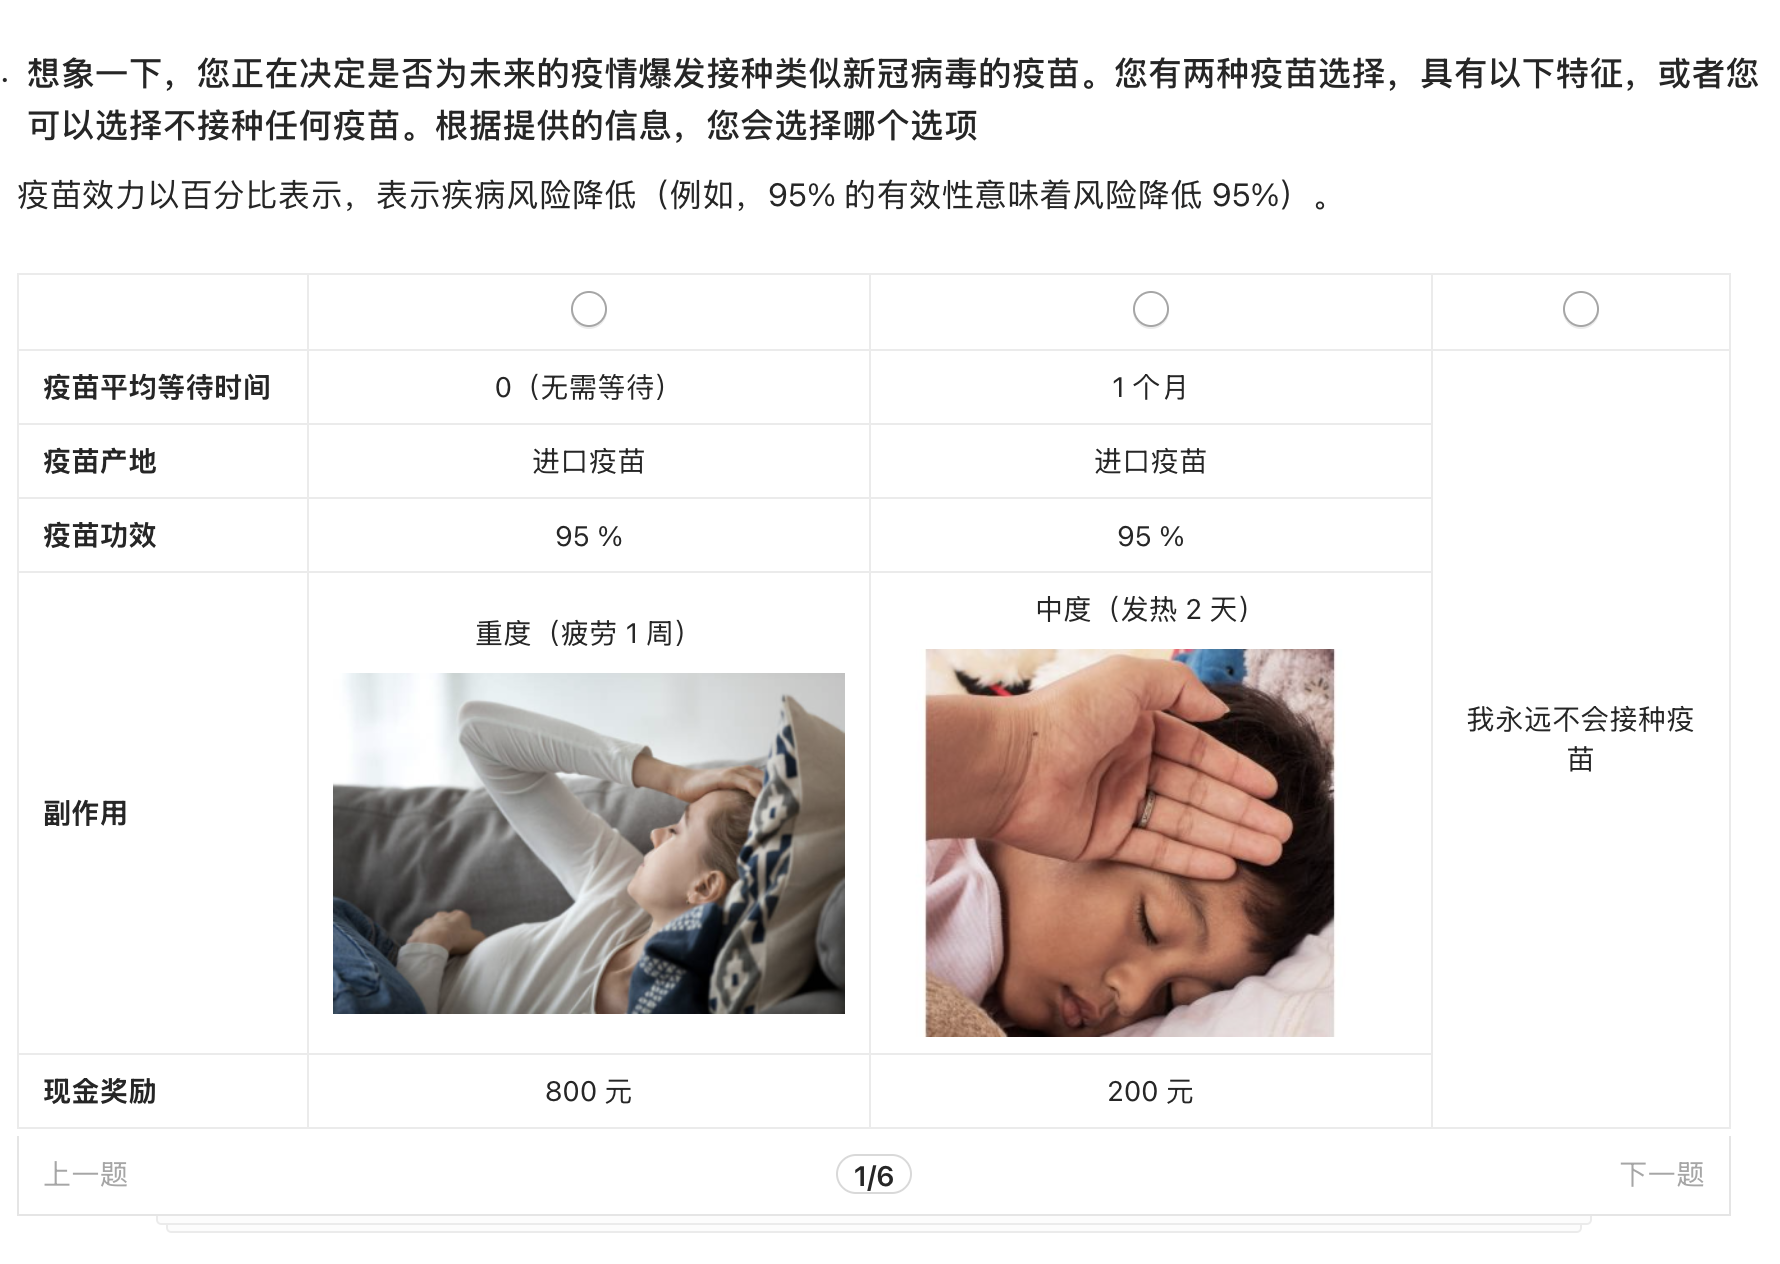
\includegraphics[width=0.9\linewidth]{sample_card.png}}{\fbox{Missing file: sample_card.png}}
    \caption{Final choice card format (illustrative).}
\end{figure}

\subsection*{B3. Experimental design}

The design was generated using the automated design feature of the Wenjuanxing survey platform based on the attribute levels in B2, yielding eight design versions. Every respondent was randomly assigned to one version and completed 6 choice sets (one set per task), each presenting two vaccine profiles (A, B) and an opt-out (``None of these''). Table~\ref{tab:design_versions} reports the number of respondents assigned to each version and the within-version attribute-level balance across the 12 non-opt-out profiles (6 sets $\times$ 2 alternatives). Versions 1--3, which together account for 69.4\% of respondents ($n = 713$), were balanced on efficacy, side-effect profile, cash incentive, and origin, and evenly represented four of the five waiting-time levels (0, 1, 3, and 6 months; the 2-month waiting level appeared only in Version 8); the remaining versions were approximately balanced. Across all eight versions, 85 unique non-opt-out profiles were administered. Fifteen of the 48 choice sets across the eight versions contained a dominated alternative pair; this is relevant to the data-quality screening described in the main text, which treated dominance violations as an inconsistency criterion. The complete 96-row fielded design matrix (8 versions $\times$ 6 tasks × 2 alternatives) is provided as a separate supplementary CSV file (\texttt{Fielded\_DCE\_Design.csv}); this Appendix B reports the version-level summary (Table~\ref{tab:design_versions}) and the complete Version~1 design matrix for illustration (Table~\ref{tab:design_matrix}).

\begin{table}[htbp]
\centering
\caption{DCE design versions: assignment and within-version attribute-level balance (counts out of 12 non-opt-out profiles per version).}
\label{tab:design_versions}
\footnotesize
\begin{tabularx}{\textwidth}{@{}l c Y Y Y Y Y@{}}
\hline
Version & $n$ & Wait 0/1/2/3/6 & Eff 50/70/95 & \shortstack{SE mild/mod/\\severe} & Cash 50/200/800 & \shortstack{Domestic/\\Imported} \\
\hline
1 & 250 & 3/3/0/3/3 & 4/4/4 & 4/4/4 & 4/4/4 & 6/6 \\
2 & 241 & 3/3/0/3/3 & 4/4/4 & 4/4/4 & 4/4/4 & 6/6 \\
3 & 222 & 3/3/0/3/3 & 4/4/4 & 4/4/4 & 4/4/4 & 6/6 \\
4 & 95 & 5/4/0/0/3 & 4/4/4 & 5/6/1 & 6/1/5 & 7/5 \\
5 & 83 & 0/1/0/7/4 & 5/4/3 & 4/4/4 & 3/6/3 & 5/7 \\
6 & 80 & 3/2/0/4/3 & 4/5/3 & 4/3/5 & 3/6/3 & 6/6 \\
7 & 55 & 5/6/0/0/1 & 2/3/7 & 2/2/8 & 4/3/5 & 6/6 \\
8 & 1 & 2/3/1/3/3 & 4/4/4 & 4/4/4 & 4/4/4 & 6/6 \\
\hline
\multicolumn{7}{@{}p{\textwidth}@{}}{\footnotesize \textit{Note.} Counts are within-version frequencies of each level across the 12 non-opt-out profiles. Versions 1--3 are balanced on efficacy, side-effect profile, cash incentive, and origin, and evenly represent four of the five waiting-time levels (0, 1, 3, 6 months); Versions 4--7 deviate from balance (e.g., Version 4 omits the 2- and 3-month levels; Version 7 omits the 2-, 3-, and one of the cash levels). Version 8 is a single-respondent version differing from Version 2 in one profile (waiting time 2 months instead of 0 months); the 2-month waiting level therefore appears only in Version 8.}
\end{tabularx}
\end{table}

The complete design matrix for Version 1 (the largest version, $n = 250$) is:

\begin{table}[H]
\centering
\caption{Complete design matrix for Version 1 ($n=250$ respondents). Opt-out alternative available in every set.}
\label{tab:design_matrix}
\small
\begin{tabular}{clccccc}
\hline
Set & Alt & Waiting time & Efficacy & Side-effect profile & Cash & Origin \\
\hline
1 & A & 0 months & 50\% & Moderate & 200 RMB & Imported \\
1 & B & 3 months & 95\% & Moderate & 50 RMB & Domestic \\
2 & A & 3 months & 70\% & Severe & 50 RMB & Domestic \\
2 & B & 6 months & 50\% & Mild & 800 RMB & Imported \\
3 & A & 1 month & 70\% & Severe & 50 RMB & Domestic \\
3 & B & 1 month & 95\% & Moderate & 200 RMB & Domestic \\
4 & A & 0 months & 50\% & Mild & 800 RMB & Imported \\
4 & B & 6 months & 95\% & Moderate & 200 RMB & Imported \\
5 & A & 6 months & 70\% & Severe & 50 RMB & Domestic \\
5 & B & 3 months & 95\% & Mild & 800 RMB & Domestic \\
6 & A & 0 months & 70\% & Severe & 200 RMB & Imported \\
6 & B & 1 month & 50\% & Mild & 800 RMB & Imported \\
\hline
\end{tabular}
\end{table}

\noindent \textbf{Attribute-level balance (aggregate).} Across all 85 administered non-opt-out profiles, vaccine efficacy (50\%, 70\%, 95\%), side-effect profile (mild, moderate, severe), and cash incentive (50, 200, 800 RMB) each appeared nearly equally often (28--30, 27--30, and 28--29 of 85 profiles, respectively); waiting time appeared in 0, 1, 2, 3, and 6 months with frequencies 22, 22, 1, 20, and 20 (the single 2-month profile occurred in Version 8). Although 0 RMB was specified as a candidate attribute level, it was not represented in any realized version; the administered profiles contained 50, 200, and 800 RMB incentive levels. We therefore do not claim statistical efficiency for this design, and D-error diagnostics are not reported. An earlier archived design export did not correspond to the fielded instrument. The design matrix reported here was therefore reconstructed from the administered respondent-level choice records and verified against the fielded survey; it constitutes the authoritative record of the realized design.

\subsection*{B4. Sample composition and population benchmarks}

The analytic sample ($N = 1{,}027$) was compared with Wuhan adult population benchmarks using 2020 census data. The sample slightly overrepresents respondents with higher educational attainment relative to the Wuhan population. The study does not apply post-stratification weights; unweighted estimates should be interpreted as conditional on the achieved sample composition. Gender and age-group distributions were broadly consistent with population benchmarks after accounting for the sampling quotas.
\clearpage
